% !TEX TS-program = xelatex
% !TEX encoding = UTF-8

\documentclass[a4paper, 11pt, twocolumn, final]{article} % use larger type; default would be 10pt

\usepackage{default}

\defaultfontfeatures{Mapping=tex-text}
\setmainfont[Ligatures=TeX]{Linux Libertine}

% \usepackage[parfill]{parskip} % Activate to begin paragraphs with an empty line rather than an indent

\usepackage{graphicx} % support the \includegraphics command and options
\usepackage{bm}

\usepackage{chngcntr}
\counterwithin{table}{section}
\counterwithin{figure}{section}
\counterwithin{equation}{section}

\title{Reinforcement learning with Sarsa, Sarsa(λ) and a Neural Network}
\author{Student 120133998, University of Sheffield}
\date{\today}

\begin{document}

\twocolumn[{
  \begin{@twocolumnfalse}
    \maketitle
    \begin{abstract}

    This report outlines our investigations into the reinforcement learning
    problem by using an example `homing' task.  We apply the Sarsa algorithm and
    use an artificial neural network to learn Q-values, and then implement
    various extensions to the Sarsa algorithm including Sarsa(λ).  We compare
    these extensions success at learning the homing problem and tune their
    parameters.

    \end{abstract}
    \tableofcontents
    \vspace{20pt}
  \end{@twocolumnfalse}
}]

\section{Introduction} .

\section{Homing task} The task we chose to focus on was a simple goal-oriented
`homing' task: a robot is placed in a room at random, and has to make its way to
the charging station, which is at a fixed place in the room.  We modelled this
using a grid of $10\times10$ discrete positions, with the robot able to move in
the four compass directions in a single action, and its charging station placed
at position $(5, 5)$.

Each episode\footnote{Note that we choose to use the terminology of `episodes'
rather than `trials', as in \cite[p.~58]{Sutton1998}.} consists of the robot
making moves according to its policy $\pi$ until either a maximum number of
moves (here denoted $t_{max}$) is reached, or it reaches its charging station at
$(5, 5)$.

\section{Basic Sarsa algorithm} At first, we implement a basic Sarsa algorithm, as
outlined in \cite[Chapter~6]{Sutton1998} with an $\epsilon$-greedy policy.  We
follow their definition of `discounted return' (denoted $R_t$) as the sum of
expected rewards (denoted $r_t$) to be obtained under policy $\pi$, with each
future reward being geometrically discounted by a factor of $\gamma$, i.e.
\begin{align}
R_t &= r_t + \gamma r_{t+1} + \gamma^2 r_{t+2} + \ldots \nonumber \\
\text{or } R_t &= \sum_{i=0}^{\infty}{\gamma^ir_{t+i}} \\
&\text{where }0 \le \gamma < 1 \nonumber
\end{align}

(Note that in general we may relax the restriction to $0 \le \gamma \le 1$ if we
know that the sequence ($t_n$) eventually becomes 0.)

The `Q-value' of a particular state-action pair, denoted $Q^\pi(s, a)$ is the
expected discounted return after taking action $a$ when in state $s$ and
following policy $\pi$ thereafter.  The Sarsa algorithm attempts to solve the
reinforcement learning problem by estimating and refining these Q-values over
every step of a training episode; we will omit the bulk of the algorithm here
(it can be found at \cite[p.~146]{Sutton1998}), but note that the crucial step
is in updating the Q-values\footnote{This is given in a slightly different form
in \cite{Sutton1998}, but I feel this was is more demonstrative of a weighted
average of the current and `target' values.}:
\begin{equation}
Q(s, a) \leftarrow (1-\alpha)Q(s, a) + \alpha[r + \gamma Q(s', a')]
\end{equation}

$Q(s, a)$ can either be used and estimated directly, or can be generated from
some parametrised model.  Our basic approach estimates directly, but then in
\autoref{sec:ext_nn} we extend this model with an artificial neural network.

As for selecting an action, we used the $\epsilon$-greedy policy throughout this
investigation:\footnote{Although we tried implementing a softmax policy with a
Gibbs-Boltzmann distribution, we tended to agree with Sutton \& Barto that
estimating a good value for $\tau$ was difficult \cite[p.~31]{Sutton1998}, and
in any case the algorithm seemed to perform poorly with this method.}  With
probability $(1-\epsilon)$ we select the action with the best Q-value, as
estimated by Sarsa, and with proability $\epsilon$ we choose randomly between
the actions.  This allows a certain degree of `exploring' while maintaining a
general stability.

\section{Learning curves and evaluation} Before moving on to a more in-depth
discussion, we briefly define the term `learning curve': in the context of our
task, we will define it as the number of steps taken to achieve the goal (i.e.
move to position $(5, 5)$) per episode.  Since with each episode, the task is
expected to be performed increasingly more efficiently, i.e. that the number of
steps taken to reach the goal should be decreasing, we measure the effectiveness
of an algorithm or set of parameters by the steepness and eventual resting point
of the decreasing learning curve.

% TODO check the "usually S = 100" here
Presented in \autoref{fig:q1_single} are two example learning curves using the
$\epsilon$-greedy policy.  Since there is an element of randomness in
$\epsilon$-greedy, and also in the choice of initial position of the robot in
the environment, the learning curve itself is non-deterministic.  To mitigate
this uncertainty, we typically average our values over a number of runs; in this
investigation we denote this number $S$ and usually take $S = 100$.  In
\autoref{fig:q1_avg} is shown an average learning curve with the same parameters
as in \autoref{fig:q1_single}, with $S = 100$ and error bars shown.  All further
learning curve graphs in this report will be of averaged learning
curves.\footnote{This answers Question 1.}

\begin{figure}
  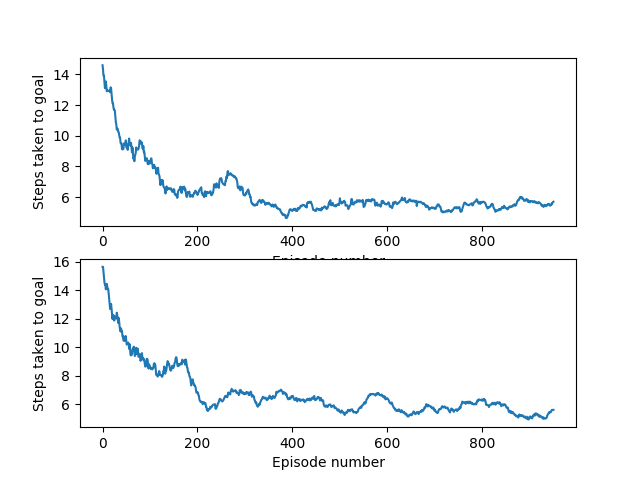
\includegraphics[width=0.49\textwidth]{figures/q1_figure_single.png}
  \caption{Two learning curves, 100-point moving average}
  \label{fig:q1_single}
\end{figure}

\begin{figure}
  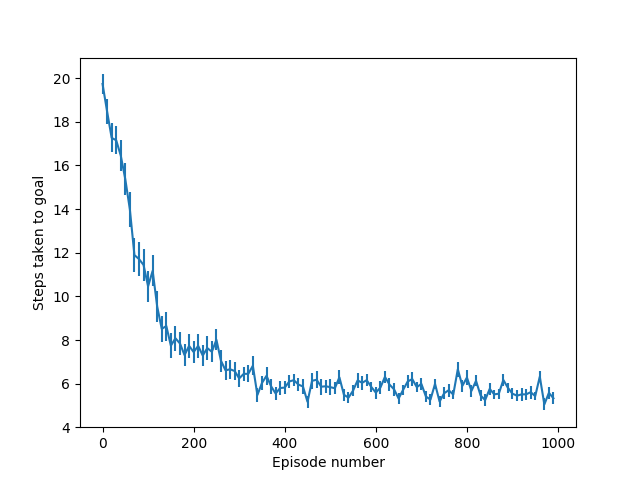
\includegraphics[width=0.49\textwidth]{figures/q1_figure_avg.png}
  \caption{Average learning curve, sampled every 10 data points}
  \label{fig:q1_avg}
\end{figure}

\section{Extensions} In this section, we attempt to build on our established
Sarsa model with various extensions, including using an artificial neural
network (abbreviated as ANN hereafter) to generate Q-values.  Since using an ANN
was suggested in the assignment brief, we use the above basic learning model
\textbf{with} the ANN as our baseline against which we will measure the other
extensions.

\subsection{Neural network} \label{sec:ext_nn} For our ANN, we use a simple
1-layer model with no hidden neurons, where there is one input neuron per state
(i.e. per position in the room), and one output neuron for each action to take.
The synapse weights are adjusted as per the above Sarsa rule for adjusting the
Q-values.  Comparing this method with the basic method at first sight gives
disappointing results---the ANN-backed model actually performs substantially
worse than the basic model above (see
\autoref{fig:ext_basic_vs_nn_vs_eligibility}).  However, as we will see, when an
eligibility trace is added this situation is reversed.

\subsection{Eligibility trace (TD(λ))} Whereas the standard Sarsa algorithm
updates each value of $Q(s, a)$ for $s = s_t$ and for all $a \in \mathcal{A}_s$
only to be closer to the `target' value of $r + \gamma Q(s', a')$, if we add an
eligibility trace to this, the Q-values for \textit{all} states are adjusted
similarly, but in proportion to the time they were most recently visited (i.e.
their `eligibility').  When an eligibility trace is added to Sarsa in this way,
it becomes known as Sarsa(λ).

As suggested by the assignment brief, we implemented an eligibility trace to
both our basic model and our ANN-backed model.  The results were successful, as
can be seen again in \autoref{fig:ext_basic_vs_nn_vs_eligibility}.\footnote{This
answers question 2.}

\begin{figure}
  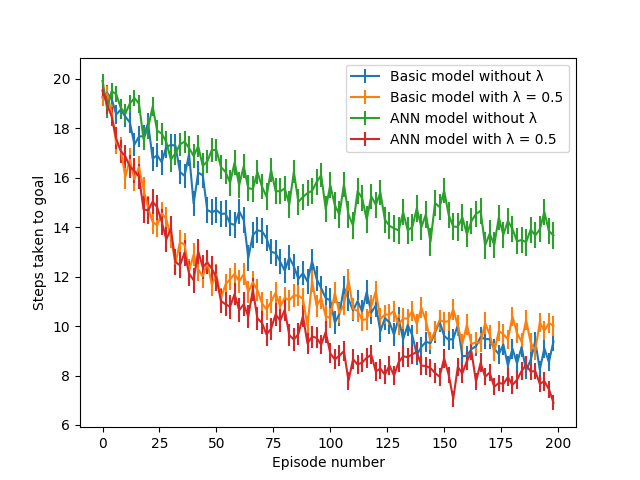
\includegraphics[width=0.49\textwidth]{figures/basic_vs_nn_vs_eligibility.png}
  \caption{Learning curves for the basic model vs. ANN model vs. using an
  eligibility trace.}
  \label{fig:ext_basic_vs_nn_vs_eligibility}
\end{figure}

\subsection{Decaying $\epsilon$} Another extension we implement is simply
letting the value of $\epsilon$ in the $\epsilon$-greedy policy decay over time.
We establish a rule, with $n$ being the episode number in the run, of
\begin{equation}
  \epsilon_n = \frac{\epsilon_0}{n}
\end{equation}
where $\epsilon_0$ is a parameter for the initial value of $\epsilon$.  As can
be seen in \autoref{fig:ext_epsilon_vs_decay}, this made little impact on the
learning curves.


\begin{figure}
  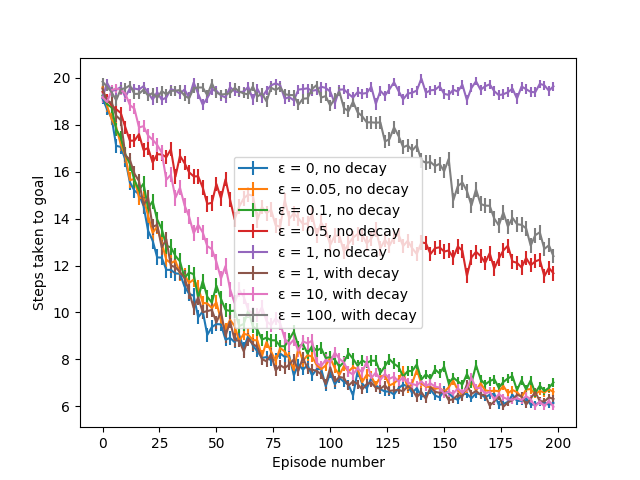
\includegraphics[width=0.49\textwidth]{figures/epsilon_decay.png}
  \caption{Learning curves for the $\epsilon$-greedy policy; plain vs. decaying
  $\epsilon$}
  \label{fig:ext_epsilon_vs_decay}
\end{figure}

\subsection{Extended actions} .

\section{Parameter tuning} .

\subsection{Representation of weights} .

\section{Limits of the model} .

\bibliographystyle{IEEEtran}
\bibliography{report}

\onecolumn \appendix

\section{Tables}
\begin{table}[H]
  \centering
  \begin{tabular}{c | c c c c c c c c c c c c}
    \hline
    & $S$ & $E$ & $t_{max}$ & $\epsilon$ decaying? & $\epsilon$ & $\alpha$ &
      $\gamma$ & Trace? & $\lambda$ & ANN? \\
    \hline
    \autoref{fig:q1_single} & N/A & 1000 & 20 & No & 0.001 & 0.1 & 0.1 & No &
      N/A & No \\
    \autoref{fig:q1_avg} & 100 & 1000 & 20 & No & 0.001 & 0.1 & 0.1 & No &
      N/A & No \\
    \autoref{fig:ext_basic_vs_nn_vs_eligibility} & 200 & 200 & 20 & No & 0.2
      & 0.8 & 0.6 & $*$ & $*$ & No \\
    \autoref{fig:ext_epsilon_vs_decay} & 100 & 200 & 20 & $*$ & $*$ & 0.8 & 0.6
      & No & N/A & Yes \\
    \hline
  \end{tabular}
  \caption{Parameters for figures generated.}
  \label{tab:parameters}
\end{table}

\begin{itemize*}
  \item $S$ denotes the number of runs that the figure is averaged over
  \item $E$ denotes the number of episodes used in each run
  \item $t_{max}$ denotes the maximum number of steps in any episode
  \item `$\epsilon$ decaying?' denotes whether a decaying $\epsilon$-greedy
    policy was used
  \item $\epsilon$ is the parameter of the $\epsilon$-greedy model
  \item $\alpha$ is the learning rate
  \item $\gamma$ is the discount rate
  \item `Trace?' denotes whether an eligibility trace was used
  \item $\lambda$ is the trace decay rate
  \item `ANN?' denotes whether an artificial neural network was used
  \item $*$ is used when parameter varies within the figure
\end{itemize*}

\begin{table}[H]
  \centering
  \begin{tabular}{r | c c c c c c c c c c}
    \hline
      & 0 & 1 & 2 & 3 & 4 & 5 & 6 & 7 & 8 & 9 \\
    \hline
    0 & → & ↓ & ↓ & ↓ & → & ↓ & ↓ & ← & ← & ↓ \\
    1 & ↓ & ↓ & ↓ & ↓ & ↓ & ↓ & ↓ & ← & ↓ & ↓ \\
    2 & ↓ & ↓ & ↓ & ↓ & ↓ & ↓ & ↓ & ↓ & ← & ↓ \\
    3 & ↓ & → & ↓ & ← & ↓ & → & ↓ & ← & ↓ & ↓ \\
    4 & ↓ & ↓ & → & ↓ & ↓ & ↓ & ↓ & ↓ & ← & ← \\
    5 & → & → & → & → & → & \colorbox{pink}{↓} & ← & ← & ↑ & ← \\
    6 & ↑ & → & → & ↑ & ↑ & ↑ & ↑ & ↑ & ← & ← \\
    7 & → & → & ↑ & ← & ↑ & → & ↑ & ← & ← & ← \\
    8 & → & ↑ & ↑ & → & → & → & ↑ & ↑ & ← & ↑ \\
    9 & ↑ & ↑ & ↑ & → & ↑ & ↑ & ↑ & ← & ↑ & ↑ \\
    \hline
  \end{tabular}
  \caption{Directions}
  \label{tab:computed_directions}
\end{table}

\section{Code snippets} \label{sec:code}

\end{document}
% Disable intented paragraphs and add space between them instead.
% \setlength{\parskip}{10pt}
% \setlength{\parindent}{0pt
